\documentclass[11pt,]{article}
\usepackage{mathpazo}
\usepackage{amssymb,amsmath}
\usepackage{ifxetex,ifluatex}
\usepackage{fixltx2e} % provides \textsubscript
\ifnum 0\ifxetex 1\fi\ifluatex 1\fi=0 % if pdftex
  \usepackage[T1]{fontenc}
  \usepackage[utf8]{inputenc}
\else % if luatex or xelatex
  \ifxetex
    \usepackage{mathspec}
    \usepackage{xltxtra,xunicode}
  \else
    \usepackage{fontspec}
  \fi
  \defaultfontfeatures{Mapping=tex-text,Scale=MatchLowercase}
  \newcommand{\euro}{€}
\fi
% use upquote if available, for straight quotes in verbatim environments
\IfFileExists{upquote.sty}{\usepackage{upquote}}{}
% use microtype if available
\IfFileExists{microtype.sty}{%
\usepackage{microtype}
\UseMicrotypeSet[protrusion]{basicmath} % disable protrusion for tt fonts
}{}
\usepackage{graphicx}
\makeatletter
\def\maxwidth{\ifdim\Gin@nat@width>\linewidth\linewidth\else\Gin@nat@width\fi}
\def\maxheight{\ifdim\Gin@nat@height>\textheight\textheight\else\Gin@nat@height\fi}
\makeatother
% Scale images if necessary, so that they will not overflow the page
% margins by default, and it is still possible to overwrite the defaults
% using explicit options in \includegraphics[width, height, ...]{}
\setkeys{Gin}{width=\maxwidth,height=\maxheight,keepaspectratio}
\ifxetex
  \usepackage[setpagesize=false, % page size defined by xetex
              unicode=false, % unicode breaks when used with xetex
              xetex]{hyperref}
\else
  \usepackage[unicode=true]{hyperref}
\fi
\hypersetup{breaklinks=true,
            bookmarks=true,
            pdfauthor={Matthew A. Barbour\^{}\{1,2,\textbackslash{}ast\}},
            pdftitle={Predicting the effects of character displacement on food-web dynamics},
            colorlinks=true,
            citecolor=blue,
            urlcolor=black,
            linkcolor=black,
            pdfborder={0 0 0}}
\urlstyle{same}  % don't use monospace font for urls
\setlength{\parindent}{0pt}
\setlength{\parskip}{6pt plus 2pt minus 1pt}
\setlength{\emergencystretch}{3em}  % prevent overfull lines
\setcounter{secnumdepth}{0}

%%% Use protect on footnotes to avoid problems with footnotes in titles
\let\rmarkdownfootnote\footnote%
\def\footnote{\protect\rmarkdownfootnote}


  \title{Predicting the effects of character displacement on food-web dynamics}
    \author{Matthew A. Barbour\(^{1,2,\ast}\)}
    \date{}
  
%%% From AmNat_MS_template.tex
%\documentclass[11pt]{article}
%\usepackage[sc]{mathpazo} %Like Palatino with extensive math support
\usepackage{fullpage}
%\usepackage[authoryear,sectionbib,sort]{natbib}
\linespread{1.7}
%\usepackage[utf8]{inputenc}
\usepackage{lineno}

%%%%%%% Sections not currently working properly
%\usepackage{titlesec}
%\titleformat{\section}[block]{\Large\bfseries\filcenter}{\thesection}{1em}{}
%\titleformat{\subsection}[block]{\Large\itshape\filcenter}{\thesubsection}{1em}{}
%\titleformat{\subsubsection}[block]{\large\itshape}{\thesubsubsection}{1em}{}
%\titleformat{\paragraph}[runin]{\itshape}{\theparagraph}{1em}{}[. ]\renewcommand{\refname}{Literature Cited}

%%% My added packages
%\usepackage{amsmath} % for matrices
%\usepackage{graphicx} % for organizing figures
%\usepackage{lmodern} % for tilde
%\usepackage[T1]{fontenc} % for tilde

%%%%%%%%% Previous - likely useful though
%\usepackage{setspace}\doublespacing
%\usepackage{float}
%\let\origfigure\figure
%\let\endorigfigure\endfigure
%\renewenvironment{figure}[1][2] {
%    \expandafter\origfigure\expandafter[H]
%} {
%    \endorigfigure
%}

\begin{document}

\maketitle


\noindent 1. University of British Columbia, Department of Zoology,
Vancouver, BC V6T 1Z4, Canada;

\noindent 2. University of Zurich, Department of Evolutionary Biology
and Environmental Studies, Winterthurerstrasse 190, 8057 Zurich,
Switzerland;

\(^\ast\) Corresponding author; e-mail:
\href{mailto:matthew.barbour@ieu.uzh.ch}{\nolinkurl{matthew.barbour@ieu.uzh.ch}}

\bigskip

\emph{Manuscript elements}: Figure 1, figure 2, figure 3, figure 4. All
figures should be printed in color.

\bigskip

\emph{Keywords}: competition; eco-evolutionary dynamics; ecological
speciation; three-spine stickleback; zooplankton

\bigskip

\emph{Manuscript type}: Note.

\bigskip

\footnotesize Prepared using an \emph{Am. Nat.} inspired \LaTeX{}
template for Rmarkdown. \normalsize

\linenumbers{} \modulolinenumbers[3]

\newpage

\section{Abstract}\label{abstract}

Ecological character displacement is a key driver of diversification and
adaptive radiation; however, there has been little work examining the
consequences of character displacement on the dynamics of ecological
communities. Given the growing recognition for the role of evolution in
structuring ecological communities, understanding how major evolutionary
processes impact ecological dynamics is increasingly important. Here, we
build a mathematical model to predict how exploitative competition
between two consumers for two resources affects the evolution of
consumer attack rates, and, in turn, consumer-resource population
dynamics. Our model suggested that increasing ecological character
displacement decreases the equilibrium density of resources, and with
sufficient divergence, results in more oscillatory (destabilizing)
consumer-resource dynamics. These results suggest that ecological
character displacement can eventually have a negative feedback on
food-web persistence in the absence of other processes.

\newpage

\section{Introduction}\label{introduction}

Ecological character displacement is thought to be a key evolutionary
process generating biodiversity (Dolph Schluter 2000; D. W. Pfennig and
Pfennig 2010; but see Stuart and Losos 2013). Ecological character
displacement describes the ``process of phenotypic evolution in a
species generated or maintained by {[}exploitative{]} resource
competition with one or more coexisting species'' (Dolph Schluter 2000).
Over the past 40 years, a large body of theoretical (e.g. Lawlor and
Smith 1976; P A Abrams 1986; Doebeli 1996; Taper and Chase 1985) and
empirical (reviewed in: Dolph Schluter 2000; Dayan and Simberloff 2005;
Stuart and Losos 2013) work has been generated to understand the
scenarios under which exploitative competition for resources leads to
the divergence of consumer foraging traits. The general result emerging
from these studies is that, if resources are nutritionally substitutable
(Peter A Abrams 1987; Fox and Vasseur 2008) and there is no other strong
source of density dependence acting on consumers (P A Abrams 1986), then
resource competition drives the divergence of consumer foraging traits
{[}Lawlor and Smith (1976); Taper and Chase (1985)). This process is not
simply driven by ecological differences, but creates an eco-evolutionary
feedback that drives further differentiation. This insight was clearly
by theoretical models that highlighted the importance of explicitly
including resource dynamics as a mediator of competition in driving
evolutionary change (Lawlor and Smith 1976; P A Abrams 1986; Taper and
Chase 1985).

Although character displacement is the result of an eco-evolutionary
feedback, the ecological consequences of this process have received
surprisingly little attention (Germain et al. 2018). Perhaps this is
because early theoretical work suggested that character displacement was
a potent stabilizing force in ecological communities (Lawlor and Smith
1976). This ecological outcome is also an intuitive one ---character
divergence reduces interspecific competition between consumers,
promoting coexistence. However, inferences about the effect of character
displacement, like the process itself, can only be made when comparing
communities in the presence and absence of competition (criteria \#3 for
character displacement, D Schluter and McPhail 1992; Dolph Schluter
2000). Current inferences about the stabilizing effects of consumer
divergence are only comparisons about communities where there are two
consumers, and even though, the focus is only on the stable coexistence
of consumer species.

The consequence of this eco-evolutionary feedback for consumer
coexistence has been well characterized (Lawlor and Smith 1976;
Germain's work). Ecological character displacement has typically been
considered to be a stabilizing factor in communities (Lawlor and Smith
1976). This is because divergence in foraging traits is thought to
reduce the strength of interspecific competition between consumers.
Reducing the strength of interspecific competition relative to
intraspecific competition is a stabilizing force in consumer-resource
systems. Consumer specialization on distinct resources suggests that
there are niche differences between consumers. Mathematically, this is
also often assumed to be the case, because using techniques such as
evolutionary invasion analysis describe the ability for a consumer with
a mutant allele to increase in abundance when rare, a demographic
signature of niche differentiation. Therefore, if both consumers are
able to invade when rare, then this suggests that they can coexist.

Character displacement involves evolutionary shifts in character states
in response to competition (D Schluter and McPhail 1992; Dolph Schluter
2000). Theoretically, this is determined by comparing character changes
in the presence and absence of a competitor. Empirically, this is
determined by meeting several criteria that rule out other possible
explanations (D Schluter and McPhail 1992; Dolph Schluter 2000).
Importantly, current inferences about the effect of character
displacement on community stability do not meet this critera. For
example, the inference that character displacement enhances species
coexistence is only made in a scenario where consumers are competing.
This type of stability is important, but it does not enable us to
examine the effect of character displacement on community stability. As
a consequence, I argue that the effect of character displacement on
community stability remains an open question.

Indeed, ecological character displacement often results in the evolution
of characters that enhance a consumer's ability to capture resources,
which tends to destabilize consumer-resource interactions (Murdoch et
al. 2003; McCann 2011). This occurs because increases in a consumer's
attack rate results in the resource being suppressed well below its
carrying capacity, which if sufficient enough, can generate
oscillations, and hence less stable, consumer-resource dynamics
(Rosenzweig 1971; Murdoch et al. 2003). Experimental decreases in
interaction strength between consumers and resources has been shown to
promote coexistence between consumers and resources (Luckinbill 1973).
Moreover, there is broad support that specialized consumers, since they
are tightly coupled to their resources, tend to exhibit
consumer-resource cycles, whereas this is not the case for generalists
(Murdoch et al. 2002). Therefore, although evolutionary responses to
exploitative competition may reduce the strength of interactions between
consumers, they ultimately increase the strength of interactions with
their resources which can destabilize the direct consumer-resource
interaction (rather than the indirect consumer-consumer interaction).
While prior models of character displacement have included more
realistic functional responses and spatial relationships between
consumers and resources, they have focused more on whether these factors
alter patterns of character displacement rather than the effects of
character displacement on the stability of the ecological community. As
a consequence, it is currently unclear whether ecological character
displacement has a net stabilizing or destabilizing effect on ecological
communities.

Here, I address this knowledge gap by building a mathematical model to
examine how ecological character displacement affects consumer-resource
dynamics in a food web context. I address two question: (1) How does
ecological character displacement affect resource abundances? (2) How
does character displacement affect food-web stability? I show that the
consequences of character displacement on food-web dynamics are not
intuitive and depend critically on the foraging scenario and tradeoff in
consumer attack rates.

\section{Methods and Results}\label{methods-and-results}

\subsection{Model of resource
competition}\label{model-of-resource-competition}

To examine how ecological character displacement affects
consumer-resource interactions and food-web dynamics, I analyzed a
continuous-time model of two consumers (\(C_1,C_2\)) competing for two
shared resources (\(R_1,R_2\)):

\[\frac{dR_1}{dt}=r_1K_1(1-\frac{R_1}{K_1})-F_{11}(R_1)C_1-F_{21}(R_1)C_2\]
\[\frac{dR_2}{dt}=r_2K_2(1-\frac{R_2}{K_2})-F_{12}(R_2)C_1-F_{22}(R_2)C_2\]
\[\frac{dC_1}{dt}=e_{11}F_{11}(R_1)C_1+e_{12}F_{12}(R_2)C_1-m_1C_1\]
\[\frac{dC_2}{dt}=e_{21}F_{21}(R_1)C_2+e_{22}F_{22}(R_2)C_2-m_2C_2\]

where \(r_i\) represents the intrinsic growth rate of resource \(i\),
\(K_i\) represents the carrying capacity of resource \(i\), \(e_{ji}\)
represents the conversion efficiency of resource \(i\) into consumer
\(j\), and \(m_j\) represents the mortality rate of consumer \(j\).
\(F_{ji}(R_i)\) represents consumer \(j\)'s feeding rate
(i.e.~functional response) on resource \(i\). This model is a useful
characterization of a scenario where consumers compete for two distinct
resources (e.g.~zooplankton and benthic invertebrates) rather than if
resources are better characterized by a continuous trait distribution
(e.g.~seed size, see Taper and Chase (1985) for an example). In the
scenario where consumer feeding rates increase linearly with resource
density, such that \(F_{ji}(R_i)=a_{ji}R_i\) where \(a_{ji}\) is the
attack rate of consumer \(j\) on resource \(i\), then this model becomes
MacArthur's model of resource competition (MacArthur (1972)). The
evolution of consumer attack rates in this model (and several
extensions) have been analyzed in detail (Lawlor and Smith (1976); P A
Abrams (1986)). The general result of these analyses is that divergent
character displacement in attack rates is an inevitable outcome of
resource competition.

Here, I examine the effects of this inevitable divergence in attack
rates on food-web dynamics. In particular, I examine how divergence in
attack rates affect resource densities as well as the local stability of
both resources and consumers. I do this by (i) deriving analytical
expressions for the relationship between attack rates and food-web
dynamics in different foraging scenarios and (ii) simulating the effects
of competition on the eco-evolutionary dynamics of consumers and
resources. For these simulations, I used an Adaptive Dynamics approach.
At each evolutionary time step, I created a mutant consumer by randomly
choosing a consumer and modifying its attack rate on one resource by
either subtracting or adding a small constant with equal probability.
The mutant's attack rate on the other resource was determined by the
shape of the tradeoff (details below). Assuming this mutant consumer is
rare, I then determined whether the mutant had higher relative fitness
than the resident consumer, and thus could invade and replace the
resident consumer. If the mutant was able to invade, I updated the
attack rate of the resident consumer to the mutant attack rate and
allowed consumer and resource dynamics to reach a steady state. I then
repeated the simulation up to 10,000 times, which was sufficient for
consumers to either reach an evolutionary stable strategy (ESS, Smith
and Price (1973)) or an evolutionary limit (e.g.
\(\frac{a_{ii}}{a_{ii}+a_{ij}}\) is constrained to a maximum of 1 and
minimum of 0).

\subsection{Resource densities}\label{resource-densities}

I start by examing the effects of character displacement on the density
of resources at equilibrium, which will set the stage for a later
analysis of food-web stability. In particular, I examine two different
foraging scenarios: one where consumers forage for both resources
simultaneously (e.g. MacArthur (1972)) and one where they cannot because
resources occur in distinct habitats (e.g. Lawlor and Smith (1976); K S
McCann, Rasmussen, and Umbanhowar (2005)). I say consumers have
undergone divergent character displacement if there evolved attack rates
are more specialized, defined as \(|\frac{a_{ii}}{a_{ii}+a_{ij}}-0.5|\),
when evolving with a competing consumer.

\textbf{Consumers forage for both resources simultaneously}: An inherent
assumption in MacArthur's model of resource competition is that
consumers can forage for both resources simultaneously. In essence, this
implies that both resources occur within the same habitat. To gain
analytical insight to this scenario, I assume that resources are
equivalent (\(r=r_1=r_2\) and \(K=K_1=K_2\)) as well as consumers
(\(e=e_{11}=e_{12}=e_{21}=e_{22}\); \(m=m_1=m_2\)), except that consumer
attack rates are mirror images of each other (\(a_{ii}=a_{11}=a_{22}\);
\(a_{ij}=a_{12}=a_{21}\)). While this scenario is arguably simplistic,
it isolates the effect of character displacement rather than any
dependence on inherent differences in consumers or resources. I show
that when both consumers and resources are present that the density of
resources at equilibrium are equivalent (\(R=R_1=R_2\)) and are
determined by the following equation (\emph{Mathematica} file with
derivation available upon request):

\[\hat{R}=\frac{1}{a_{ii}+a_{ij}}\cdot\frac{m}{e}\] Note that a key
determinant of resource density is the consumer's total attack rate,
\(a_{ii}+a_{ij}\). Since the total attack rate is in the denominator,
this implies that resource densities will decrease if evolution favors
an increase in total attack rate. I assume that consumers are not
`Darwinian demons' (Law (1979)) and thus the evolution of their attack
rates are subject to certain constraints. I modelled these constraints
such that \(\big(a_{ii}/{A}\big)^n+\big(a_{ij}/{A}\big)^n=1\), where
\(A\) is the total investment in attack rates and \(n\) describes the
shape of the tradeoff (Sargent and Otto (2006)). This function has the
useful property that it differentiates between cases where intermediate
combinations of \(a_{ii}\) and \(a_{ij}\) are higher, on average, than
the extremes (when \(n>1\), green line in Fig. \ref{fig:Tradeoff}) or,
conversely, where the two extremes are higher, on average, than
intermediate investments (when \(n<1\), orange line Fig.
\ref{fig:Tradeoff}). When \(n=1\), the tradeoff function is linear, and
all combinations of \(a_{ii}\) and \(a_{ij}\) have the same total attack
rate (blue line in Fig. \ref{fig:Tradeoff}).

\begin{figure}
\centering
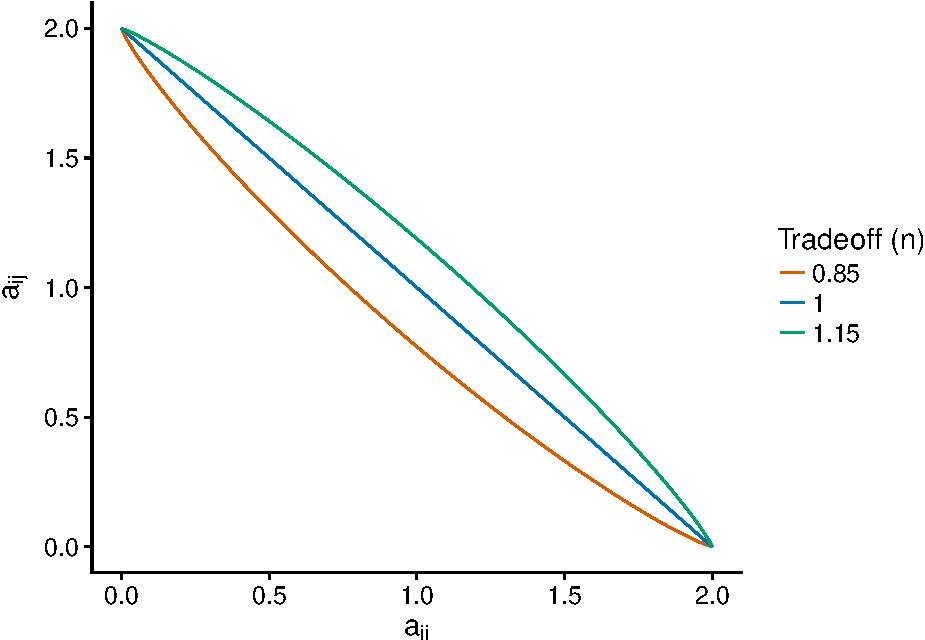
\includegraphics{ECD_Supp_Mat_files/figure-latex/Tradeoff-1.pdf}
\caption{\label{fig:Tradeoff}Tradeoff forms for consumer attack rates.}
\end{figure}

Previous work has shown that consumers undergo divergent character
displacement regardless of the shape of the tradeoff (Lawlor and Smith
(1976); P A Abrams (1986)). Interestingly, I find that the shape of the
tradeoff qualitatively affects the relationship between character
displacement and resource density (Fig. \ref{fig:MacArthur_Resources}).
For example, if consumer's are constrained by a linear tradeoff (blue
lines), then there is no net change in total attack rate (Fig.
\ref{fig:MacArthur_Resources}A) and character displacement has no effect
on resource densities (Fig. \ref{fig:MacArthur_Resources}B). If the
tradeoff is concave down (green lines), then resource abundances can
actually increase under character displacement (Fig.
\ref{fig:MacArthur_Resources}B). This is because the total attack rate
of consumers is maximized at intermediate values (\(a_{ii}=a_{ij}\)) and
decreases as consumers diverge (Fig. \ref{fig:MacArthur_Resources}A).
Note that detecting this effect in nature would likely be difficult,
since a concave-down tradeoff results in relatively small displacement
relative to other tradeoff shapes (Lawlor and Smith (1976); green points
in Fig. \ref{fig:MacArthur_Resources}A,B). When the tradeoff is concave
up (orange lines), character displacement suppresses resource densities
due to the increase in total attack rates (Fig.
\ref{fig:MacArthur_Resources}A,B). Although the equation I derived for
resource density was for the scenario where both consumers and both
resources are present, it predicts well the density of resources when a
single consumer reaches its ESS (triangles on respective colored lines
in Fig. \ref{fig:MacArthur_Resources}B). This is because a single
consumer evolves to be a generalist that has equal attack rates on each
resource (triangles at 0.5 along x-axis in Fig.
\ref{fig:MacArthur_Resources}A), resulting in equivalent resource
densities.

\begin{figure}
\centering
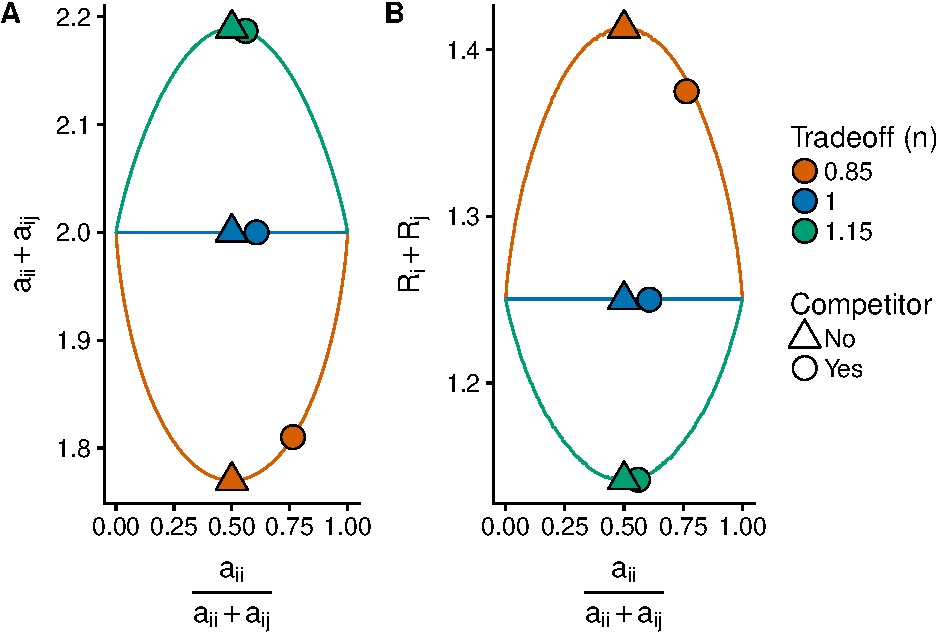
\includegraphics{ECD_Supp_Mat_files/figure-latex/MacArthur_Resources-1.pdf}
\caption{\label{fig:MacArthur_Resources}Effect of character displacement
on total attack rates (A) and resource densities (B) when consumers can
forage for both resources simultaneously.}
\end{figure}

\textbf{Consumers \emph{cannot} forage for both resources
simultaneously}: Most models of character displacement have assumed a
scenario where consumers can forage for both resources simultaneously
(e.g. Taper and Chase (1985); P A Abrams (1986)). This assumption may be
valid for some foraging scenarios (e.g.~Darwin's finches foraging for
seeds); however, in many situations consumers forage for resources that
occur in different habitats, and thus cannot forage for both
simultaneosly. The only character displacement model that I am aware of
that modeled resources in different habitats was one examined by Lawlor
and Smith (1976). This model takes the same form as the previous model,
except now the consumer's feeding rate takes the form:

\[F_{ji}(R_i)=w_{ji}a_{ji}R_i\]

where \(w_{ji}\) represents the proportion of time consumer \(j\) spends
foraging in a habitat where only resource \(j\) is found (i.e.~habitat
preference). Note that since \(w_{ji}\) is a proportion that
\(w_{jj}=1-w_{ji}\). As with attack rates, I assume that consumer
habitat preferences are mirror images of each other
(\(w=w_{11}=w_{22}\)).

Lawlor and Smith (1976) found that consumers still underwent divergent
character displacement regardless of whether consumers could or could
not forage for resources simultaneously. I find that the foraging
scenario qualitatively affects the relationship between character
displacement and resource densities. To demonstrate this, note that
again resource densities are equivalent at equilibrium (\(R=R_1=R_2\)
when both consumers and resources present), but are now determined by
the following equation (\emph{Mathematica} file with derivation
available upon request):

\[\hat{R}=\frac{1}{wa_{ii}+(1-w)a_{ij}}\cdot\frac{m}{e}\]

This equation implies that if consumers evolve to become specialists on
resources that occur in their preferred habitat (e.g. \(w>0.5\) and
\(a_{ii}>a_{ij}\)), then character displacement will always increase the
effective attack rate of consumers (\(wa_{ii}+(1-w)a_{ij}\)), regardless
of the tradeoff (Fig. \ref{fig:LS_Resources}A). Thus, character
displacement always results in resource suppression if consumers are
competing for resources that occur in different habitats (Fig.
\ref{fig:LS_Resources}B). Note that the shape of the tradeoff can modify
the effect of character displacement. This is not so much due to the
tradeoff affecting the magnitude of displacement (it does, but the
effect is minor), but because the form of the tradeoff affects resource
abundances when a single consumer has reached its ESS (triangles in Fig.
\ref{fig:LS_Resources}B). In contrast, resource densities reach a
similar value when consumers evolve in the presence of a competitor
(circles in Fig. \ref{fig:LS_Resources}B), because character
displacement tends to reach a constraint of complete specialization.

These results do lead to an interesting prediction that could be tested
either experimentally or with field data. If consumers are competing for
resources that occur in different habitats, then greater character
displacement corresponds to a greater decrease in resource densities
(line trajectories in Fig. \ref{fig:LS_Resources}B). This prediction
likely only applies to comparisons within species where there is likely
little difference in the shape of the tradeoff among populations.

It is worth noting that in this foraging scenario, resource densities
are consistently higher at the single consumer ESS compared to the
predictions I derived for when both consumers are present (deviation of
triangles from respective colored lines in Fig.
\ref{fig:LS_Resources}B). This is likely because consumers actually
evolve to be slightly specialized on the resources that occur in their
non-preferred habitat (deviation of triangles from 0.5 along x-axis in
Fig. \ref{fig:LS_Resources}B).

\begin{figure}
\centering
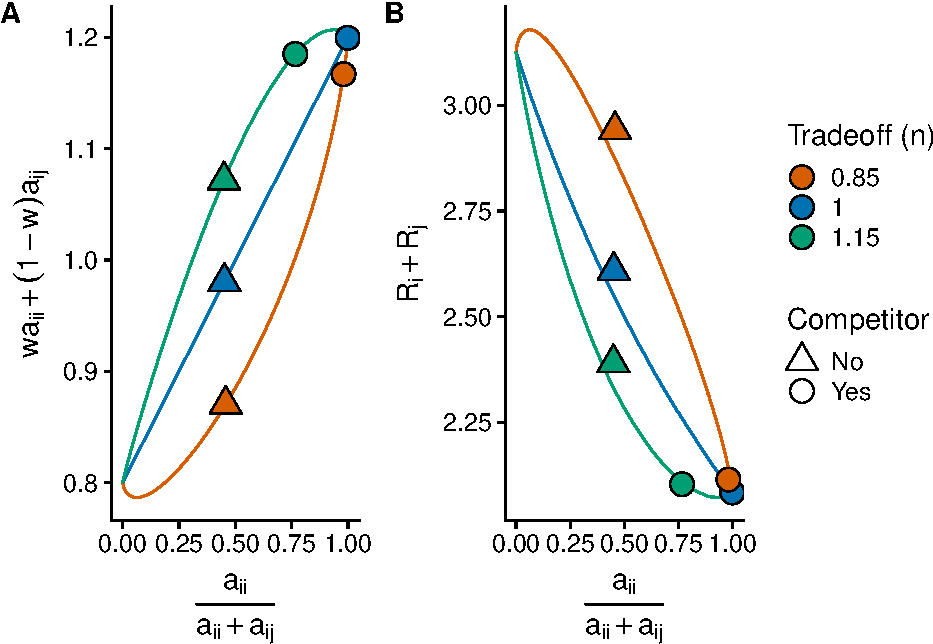
\includegraphics{ECD_Supp_Mat_files/figure-latex/LS_Resources-1.pdf}
\caption{\label{fig:LS_Resources}Effect of character displacement on
effective attack rates (A) and resource densities (B) when consumers
cannot forage for resources simultaneously.}
\end{figure}

The effect of the foraging scenario on the relationship between
character displacement and resource densities appears to be quite
general. For example, even if I consider a more realistic consumer
functional response (derived by K S McCann, Rasmussen, and Umbanhowar
(2005)):

\[F_{ii}(R_i,R_j)=\frac{a_{ii}W_{ii}R_i}{1+a_{ii}hW_{ii}R_i+a_{ij}hW_{ij}R_j}\]

where consumer feeding rates on resource \(i\) are influenced by both
resource densities; saturate as resource densities increase (due to
handling time \(h\)); and consumer habitat preferences are modified by
relative resource densities, such that:

\[W_{ii}=\frac{wR_i}{wR_i+(1-w)R_j}\]

I still observe the same qualitative relationship between character
displacement and resource suppression (Fig. \ref{fig:McCann_Resources}
in Appendix). This is because resource competition always leads to
character divergence and equilibrium resource densities are governed by
similar dynamics (\emph{Mathematica} file with derivations available
upon request):

\[\hat{R}=\frac{1}{wa_{ii}+(1-w)a_{ij}}\cdot\frac{m}{e-hm}\]

\subsection{Food-web stability}\label{food-web-stability}

Of the prior models of character displacement, only Lawlor and Smith
(1976) examine the effect of character displacement on the ecological
stability of the system. They conducted a detailed theoretical analysis
of three different metrics of stability: (i) stable coexistence of
consumers, defined as the mutual invasibility of each consumer; (ii)
global stability of consumers, defined as the continued coexistence of
both consumers when resource dynamics are perturbed; and (iii) local
stability, defined as the rate at which the four-species food web
returned to equilibrium after a small perturbation to species
abundances. Note that the first two metrics correspond to the stable
coexistence of consumers, while the third metric measures the stability
of the entire food web. Lawlor and Smith (1976) found that character
displacement enhanced the stable coexistence of consumers, yet had a
small negative effect on the local stability of the food web.

Lawlor and Smith (1976)'s work gave fundamental insight to the effect of
character displacement on ecological stability; however, none of their
stability analyses compared food webs with and without a competing
consumer. Such comparisons are necessary for inferring the effects of
ecological character displacement, a point that has been made clear in
the criteria to demonstrate character displacement (Dolph Schluter
(2000); D Schluter and McPhail (1992)). In fact, the first two metrics
of stability can only be assessed when both consumers are present
because it examines the effect of divergence on coexistence, which
requires both consumers to be present. In contrast, local stability can
be compared in food webs with and without a competing consumer, and thus
provides a useful benchmark for examining the effects of character
displacement on food-web stability.

Below, I plot the results from the same simulations I did previously
except now local stability
(\(-1\times\operatorname{Re}(\lambda_{max})\)) is on the y-axis (Fig.
\ref{fig:Stability}). In general, I find that resource supression goes
hand-in-hand with local stability, a tendency that has been noted by
others (Murdoch, Briggs, and Nisbet (2003); Kevin S McCann (2011)).
Whenever character displacement results in resource suppression, I
observe a decrease in local stability (Fig. \ref{fig:Stability}). This
is not simply a consequence of having an additional consumer in the
system, but emerges from the eco-evolutionary feedback between character
displacement and resource suppression (compare initial (small points)
with evolved strategies (large points), Fig. \ref{fig:Stability}). Note
that I reach the same fundamental conclusions when I incorporated a more
realistic functional response for the consumers (Fig.
\ref{fig:Stability_McCann} in Appendix).

\begin{figure}
\centering
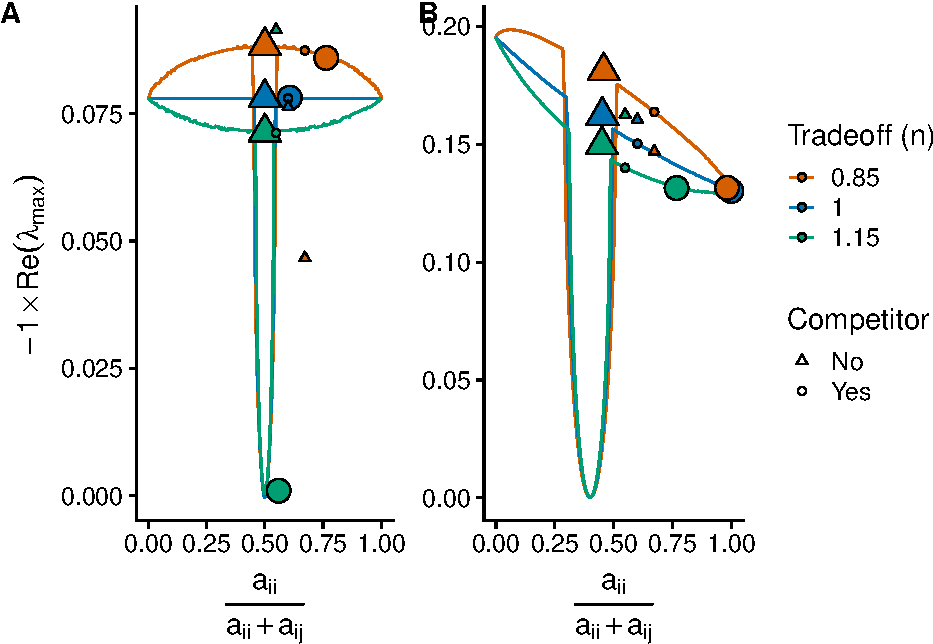
\includegraphics{ECD_Supp_Mat_files/figure-latex/Stability-1.pdf}
\caption{\label{fig:Stability}Effect of character displacement on local
stability when consumers can (A) and cannot (B) forage for both
resources simultaneously. Small and large points correspond to initial
and evolved strategies, respectively.}
\end{figure}

I conducted the previous simulations on a scenario where the food web
remains locally stable (\(\operatorname{Re}(\lambda_{max})<0\)). Is it
possible that character displacement would ever result in a locally
unstable food web? To gain analytical insight to this question, I
examined the conditions governing the local stability of the
four-species food web when consumers exhibit a more realistic functional
response (K S McCann, Rasmussen, and Umbanhowar (2005)). I show that the
four-species food web will transition from having a locally stable
equilibrium to a limit cycle under the following conditions
(\emph{Mathematica} file with derivation available upon request):

\[wa_{ii}+(1-w)a_{ij} > \frac{e+hm}{hK(e-hm)}\]

Previously, I showed that character displacement always increases the
effective attack rate of consumers (\(wa_{ii}+(1-w)a_{ij}\)), regardless
of the the shape of the tradeoff (Fig. \ref{fig:LS_Resources}A). Thus,
character displacement is capable of pushing food webs to a point where
they are locally unstable.

\section{Discussion}\label{discussion}

Important point: Criteria 5 in D Schluter and McPhail (1992) does not
make sense since character displacement usually alters resource
distributions. Think about this more.

\subsection{Predictions for threespine
stickleback}\label{predictions-for-threespine-stickleback}

The scenario where the relationship between character displacement and
resource suppression is the strongest is when the tradeoff in attack
rates is concave-up and consumers are competing for resources that occur
in different habitats (orange points in Fig. \ref{fig:LS_Resources}B and
Fig. \ref{fig:McCann_Resources}B). Prior work in threespine stickleback
suggests that the evolution of stickleback attack rates are constrained
by a concave-up tradeoff (Dolph Schluter (1993); Arnegard et al. (2014))
and that stickleback ecotypes are competing for resources that occur in
different habitats (benthic vs.~limnetic, D Schluter and McPhail
(1992)). Thus, I predict that ecological character displacement in
sticklebacks would suppress resource densities and decrease local
stability.

While measuring resource densities is relatively straightforward,
measuring stability is notoriously difficult. One of the more easy to
acquire empirical metrics of stability is the coefficient of variation
(\(CV=\frac{\sigma}{\mu}\)) as this only requires measurements of
resource (or consumer) densities over time. Interestingly, there is a
close correspondence between the coefficient of variation and the local
stability of a food web (Gellner, McCann, and Hastings (2016)). Thus, I
predict that character displacement in threespine stickleback will
increase the \(CV\) of resource (or consumer) densities.

Consumer and resource densities in these dynamical models can be
interpreted from either a population or biomass perspective (Yodzis and
Innes (1992); Murdoch, Briggs, and Nisbet (2003); Kevin S McCann
(2011)). For the stickleback system, you have data on seasonal dynamics
of resources in terms of both abundances and biomass. Within a season, I
do not expect stickleback abundances to be coupled to the abundances of
zooplankton and benthic invertebrates, given that stickleback reproduce
annually whereas zooplankton and benthic invertebrates can reproduce
many times within a season. Instead, I expect that stickleback biomass
will be coupled to the biomass of zooplankton and benthic invertebrates
within a season. This is because there will be lots of young stickleback
at the beginning of the season, and they will eat a lot of resources and
grow in size as the season progresses. If this is true, I also expect to
see the largest negative effect of stickleback on resource densities
late in the season.

\subsubsection{Other relevant points}\label{other-relevant-points}

Although I used an Adaptive Dynamics approach here, I expect that these
theoretical predictions would apply to models that assumed a different
genetic architecture of attack rates (e.g.~quantitative genetics). I
expect this because, time and time again, models that explicitly include
resource dynamics inevitably show that resource competition results in
divergent character displacement, regardless of the genetic architecture
of traits (see synthesis by Taper and Chase (1985)). Finally, my
conclusions only apply to biological resources that are nutritionally
substitutable. It would be interesting to extend these current analyses
to non-substitutable resources where convergent character displacement
is expected (Peter A Abrams (1987); Fox and Vasseur (2008)).

\subsection{Acknowledgement}\label{acknowledgement}

The content of this paper was greatly enhanced by numerous conversations
with Seth Rudman. Sally Otto provided much help in early analyses of the
mathematical model and I would not have been able to take the theory as
far as I did without her guidance and her pushing me.

\subsection{Appendix: More realistic functional
response}\label{appendix-more-realistic-functional-response}

\begin{figure}
\centering
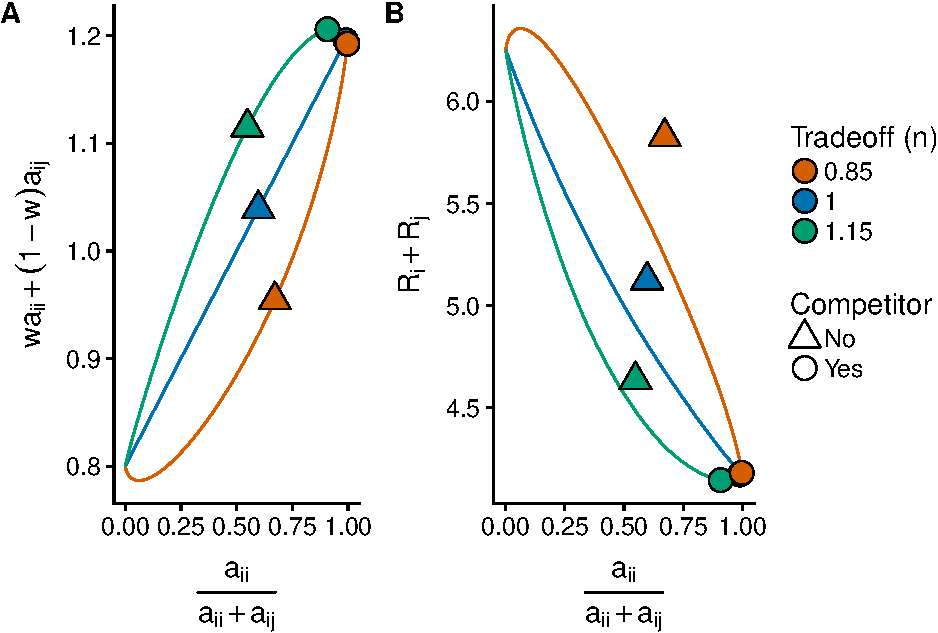
\includegraphics{ECD_Supp_Mat_files/figure-latex/McCann_Resources-1.pdf}
\caption{\label{fig:McCann_Resources}Effect of character displacement on
total attack rates (A) and resource densities (B) when consumers exhibit
a more realistic functional response.}
\end{figure}

\begin{figure}
\centering
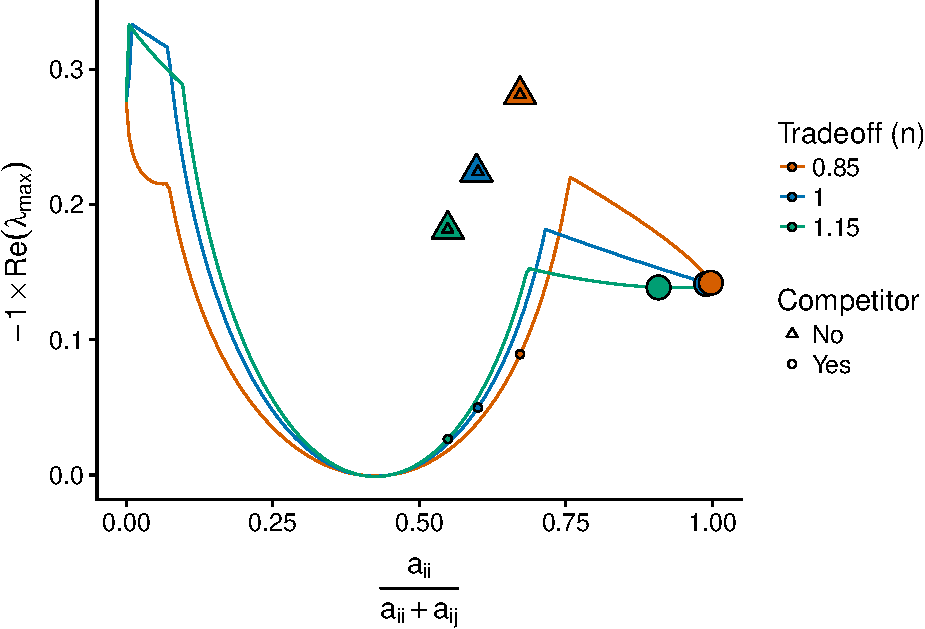
\includegraphics{ECD_Supp_Mat_files/figure-latex/Stability_McCann-1.pdf}
\caption{\label{fig:Stability_McCann}Effect of character displacement on
local stability when consumers exhibit a more realistic functional
response.}
\end{figure}

\hypertarget{refs}{}
\hypertarget{ref-Abrams1986}{}
Abrams, P A. 1986. ``Character Displacement and Niche Shift Analyzed
Using Consumer-Resource Models of Competition.'' \emph{Theor. Popul.
Biol.} 29 (1): 107--60.

\hypertarget{ref-Abrams1987}{}
Abrams, Peter A. 1987. ``Alternative Models of Character Displacement
and Niche Shift. I. Adaptive Shifts in Resource Use When There Is
Competition for Nutritionally Nonsubstitutable Resources.''
\emph{Evolution} 41 (3). Wiley Online Library: 651--61.

\hypertarget{ref-Arnegard2014}{}
Arnegard, Matthew E, Matthew D McGee, Blake Matthews, Kerry B Marchinko,
Gina L Conte, Sahriar Kabir, Nicole Bedford, et al. 2014. ``Genetics of
Ecological Divergence During Speciation.'' \emph{Nature} 511 (7509):
307--11.

\hypertarget{ref-Dayan2005}{}
Dayan, Tamar, and Daniel Simberloff. 2005. ``Ecological and
Community-Wide Character Displacement: The Next Generation.''
\emph{Ecol. Lett.} 8 (8). Blackwell Science Ltd: 875--94.

\hypertarget{ref-Doebeli1996}{}
Doebeli, Michael. 1996. ``An Explicit Genetic Model for Ecological
Character Displacement.'' \emph{Ecology} 77 (2). Ecological Society of
America: 510--20.

\hypertarget{ref-Fox2008}{}
Fox, Jeremy W, and David A Vasseur. 2008. ``Character Convergence Under
Competition for Nutritionally Essential Resources.'' \emph{The American
Naturalist} 172 (5). The University of Chicago Press: 667--80.

\hypertarget{ref-Gellner2016}{}
Gellner, Gabriel, Kevin S McCann, and Alan Hastings. 2016. ``The Duality
of Stability: Towards a Stochastic Theory of Species Interactions.''
\emph{Theor. Ecol.} 9 (4): 477--85.

\hypertarget{ref-Germain2018}{}
Germain, Rachel M, Jennifer L Williams, Dolph Schluter, and Amy L
Angert. 2018. ``Moving Character Displacement Beyond Characters Using
Contemporary Coexistence Theory.'' \emph{Trends Ecol. Evol.} 33 (2):
74--84.

\hypertarget{ref-Law1979}{}
Law, Richard. 1979. ``Optimal Life Histories Under Age-Specific
Predation.'' \emph{Am. Nat.} 114 (3): 399--417.

\hypertarget{ref-Lawlor1976}{}
Lawlor, Lawrence R, and J Maynard Smith. 1976. ``The Coevolution and
Stability of Competing Species.'' \emph{Am. Nat.} 110 (971).
{[}University of Chicago Press, American Society of Naturalists{]}:
79--99.

\hypertarget{ref-MacArthur1972}{}
MacArthur, R H. 1972. \emph{Geographical Ecology: Patterns in the
Distribution of Species}. Biology / {[}Princeton University Press{]}.
Princeton University Press.

\hypertarget{ref-McCann2005}{}
McCann, K S, J B Rasmussen, and J Umbanhowar. 2005. ``The Dynamics of
Spatially Coupled Food Webs.'' \emph{Ecol. Lett.} 8 (5). Blackwell
Science Ltd: 513--23.

\hypertarget{ref-McCann2011}{}
McCann, Kevin S. 2011. \emph{Food Webs (Mpb-50)}. Princeton University
Press.

\hypertarget{ref-Murdoch2003}{}
Murdoch, W W, C J Briggs, and R M Nisbet. 2003. \emph{Consumer-Resource
Dynamics}. Monographs in Population Biology. Princeton University Press.

\hypertarget{ref-Pfennig2010}{}
Pfennig, David W, and Karin S Pfennig. 2010. ``Character Displacement
and the Origins of Diversity.'' \emph{Am. Nat.} 176 Suppl 1 (December):
S26--44.

\hypertarget{ref-Sargent2006}{}
Sargent, Risa D, and Sarah P Otto. 2006. ``The Role of Local Species
Abundance in the Evolution of Pollinator Attraction in Flowering
Plants.'' \emph{Am. Nat.} 167 (1): 67--80.

\hypertarget{ref-Schluter1992}{}
Schluter, D, and J D McPhail. 1992. ``Ecological Character Displacement
and Speciation in Sticklebacks.'' \emph{Am. Nat.} 140 (1): 85--108.

\hypertarget{ref-Schluter1993}{}
Schluter, Dolph. 1993. ``Adaptive Radiation in Sticklebacks: Size,
Shape, and Habitat Use Efficiency.'' \emph{Ecology} 74 (3): 699--709.

\hypertarget{ref-Schluter2000}{}
---------. 2000. ``Ecological Character Displacement in Adaptive
Radiation.'' \emph{Am. Nat.} 156 (S4): S4--S16.

\hypertarget{ref-Smith1973}{}
Smith, J Maynard, and G R Price. 1973. ``The Logic of Animal Conflict.''
\emph{Nature} 246 (November). Nature Publishing Group: 15.

\hypertarget{ref-Stuart2013}{}
Stuart, Yoel E, and Jonathan B Losos. 2013. ``Ecological Character
Displacement: Glass Half Full or Half Empty?'' \emph{Trends Ecol. Evol.}
28 (7): 402--8.

\hypertarget{ref-Taper1985}{}
Taper, Mark L, and Ted J Chase. 1985. ``Quantitative Genetic Models for
the Coevolution of Character Displacement.'' \emph{Ecology} 66 (2).
Ecological Society of America: 355--71.

\hypertarget{ref-Yodzis1992}{}
Yodzis, P, and S Innes. 1992. ``Body Size and Consumer-Resource
Dynamics.'' \emph{Am. Nat.} 139 (6). {[}University of Chicago Press,
American Society of Naturalists{]}: 1151--75.

\end{document}
